% MANUSCRIPT_VERSION: 7
\documentclass{svproc}
\usepackage{url}
\usepackage{graphicx}
\usepackage{amsmath,amssymb}
\usepackage{mathptmx}
\usepackage{booktabs}
\usepackage{longtable}
\usepackage{placeins}
\setlength{\emergencystretch}{2em}
\def\UrlFont{\rmfamily}
\pdfinfo{/Title (Repetition, Information Preservation, and Decision Reliability in Hierarchical Language-Model Agents) /Author (Anonymous) /Subject (Anonymous research draft for scientific review)}

\begin{document}
\mainmatter
\title{Repetition, Information Preservation, and Decision Reliability in Hierarchical Language-Model Agents}
\titlerunning{Repetition and Information Preservation}
\author{Anonymous}
\authorrunning{Anonymous}
\institute{Anonymous submission }
\maketitle

\begin{abstract}
Language model agents often pass repeated or rephrased reports through several decision makers. Understanding whether repetition preserves useful information or changes decisions without adding evidence is essential for reliable coordination. We propose a controlled evaluation framework that separates information preservation, whether the available information determines the correct decision, and final decision accuracy. Frozen worker reports and paired scenarios containing consequential changes or harmless edits distinguish repeated presentation from fresh computation and new evidence. A held-out evaluation of Qwen3-14B and Phi-4 covers candidate schedule selection and rule-based workflows in flat and hierarchical organizations, using 192 independent base pairs shared across models, 27,648 decision trajectories, and 55,296 model calls. On scheduling, exact repetition changes accuracy by -0.17 and -1.09 percentage points, respectively, with 95\% cluster-bootstrap intervals of [-2.21, +1.74] and [-3.17, +1.00]. These small average effects conceal offsetting corrections and regressions. An audit of 6,336 development and validation summaries locates numerical information loss in raw model output, with no subsequent changes during processing or delivery. A 6 pair diagnostic illustrates that preserving information and applying it correctly are distinct challenges. A separate 48-pair study examines repetition targets and access to original reports. By combining controlled report transformations with audits of the information available to decision makers, the framework reveals reliability failures that aggregate accuracy alone can obscure. These findings provide a practical foundation for evaluating repetition and identifying where agent communication and decision processes need improvement.
% END AUTO: abstract
\keywords{language-model agents, repetition, hierarchical aggregation, information preservation, behavioral evaluation}
\end{abstract}

\section{Introduction}
Reliable coordination among language model agents depends on preserving the meaning of information as it moves between workers, managers, and final decision makers. Reports often overlap, repeat an observation, or use similar wording for different candidates, constraints, or versions. These distinctions become especially important when a manager must summarize several reports for another agent. Understanding how repetition affects this process is therefore a practical step toward building agent systems whose decisions remain grounded in the information they receive.

The challenge arises even when every original report is correct. In a scheduling team, one worker may report that a candidate finishes quickly while another identifies a violation of machine capacity. Repeating the favorable report does not make the candidate feasible, but it may help its completion time survive summarization. Repetition can therefore affect both which facts are preserved and how those facts influence a decision. Evaluating these effects requires following the information through the system and checking whether each decision is justified by the evidence available at that stage.

Existing research examines evidence duplication, source dependence, and hierarchical communication \cite{sybil,copies,scaling}. Distributed information benchmarks also demonstrate difficulties in bringing important facts into a team's discussion \cite{hidden}. Building on these directions, we introduce a controlled framework that connects report presentation, information preservation, and decision correctness. All required findings are initially delivered. A flat decision maker reads the reports directly, while a hierarchical decision maker receives summaries from two intermediate managers. Frozen worker reports separate repeated presentation from additional computation or new evidence. Executable constraints provide an independent basis for checking the correct answer, while paired scenarios test whether agents respond to consequential changes and remain consistent under harmless edits.

A central contribution is the distinction between preserving information, retaining enough information to determine the correct decision, and actually making that decision. These are related but different requirements. A missing completion time may leave the answer unchanged when only one candidate is feasible. Conversely, a model may receive every necessary comparison and still select the wrong candidate. Measuring these outcomes separately makes it possible to distinguish incomplete summaries from decisions that contradict sufficient evidence.

The main evaluation covers 192 independent base pairs shared across two models and 27,648 decision trajectories. Its scheduling results show why average accuracy alone gives an incomplete picture of repetition. Corrections and regressions largely offset, and the large benefit observed in the pilot does not generalize to the main evaluation. These findings provide a stronger empirical basis for assessing repetition than either an isolated success or a single average score. An audit of 6,336 development and validation summaries identifies numerical information loss in raw manager outputs. A focused six-pair diagnostic further illustrates how information loss and failures to apply available information can be examined separately.

Together, the benchmark, paired transformations, and trace-based analysis provide a practical method for evaluating communication reliability in agent systems. Their value lies in making failures interpretable and identifying whether improvements should target summary content, the sufficiency of delivered evidence, or its application in the final decision.





\section{Related Work}
Gao et al. \cite{copies} study restated observations in logs, web documents, and agent-written communication, including summaries and hierarchical protocols. Their team aggregator reads a roster and full log; our root receives intermediate summaries and a value-free scope registry, combining mandatory constraints with numerical objectives. Our distinction is complementary information under restricted access, not discovering evidence double counting. Bara \cite{sybil} distinguishes report multiplicity, evidence ancestry, and correlated extraction errors, motivating separate tracking of copies and verification executions.

Whole-prompt repetition can improve non-reasoning models \cite{promptrepeat}. We selectively repeat individual reports, potentially changing what managers forward, so our treatment neither directly tests nor contradicts those findings. Self-consistency samples additional reasoning paths \cite{selfconsistency}, while multiagent debate exchanges separately generated responses \cite{debate}, with benefits depending on protocol and resource comparisons \cite{smit}. These methods add computation; copying accepted reports does not. Fresh execution on the same source also does not establish independent evidence. Self-correction research similarly distinguishes repeated reasoning from external feedback \cite{selfcorrect}.

Kim et al. \cite{scaling} examine interactions between agent architecture and task structure; we use only version 3 of their preprint. HiddenBench \cite{hidden} studies exploration of distributed information and structured communication. Our replay begins after essential reports arrive, isolating aggregation from discovery. MAST \cite{mast} covers broader coordination and execution failures. Distributed fact recovery under misinformation \cite{distributed} concerns false reports, a different intervention from legitimate world changes: our main replay supplies correct reports in both worlds.

Summarization research distinguishes source faithfulness from factual correctness \cite{maynez}. FRANK separates predicate, entity, and circumstance errors \cite{frank}. Our typed scope fields support executable scoring of analogous errors, with decision sufficiency as an additional criterion. CheckList \cite{checklist} motivates behavioral tests beyond aggregate accuracy, while PAWS \cite{paws} demonstrates that lexical overlap need not imply equivalent meaning. Position effects \cite{middle} and evidence metadata \cite{metadata} offer alternative explanations for changed answers, cautioning against attributing presentation effects to source counting or hidden reasoning without corresponding interventions.




\section{Task Setting and Worked Example}

\subsection{Selecting a Feasible Candidate}

The model receives a set of candidate schedules and must choose the one that finishes earliest while satisfying every mandatory requirement. The choice is restricted to the supplied candidates. A schedule's finishing time, called its \emph{makespan}, is the time when its last job finishes.

A candidate is \emph{feasible} if it respects all applicable constraints. Jobs must follow the required order, start no earlier than their release times, stay within resource capacities, meet deadlines, and avoid periods when required resources are unavailable. Each job has an integer duration and resource demand and must run without interruption. A job starting at $s_j$ with duration $d_j$ occupies the interval $[s_j,s_j+d_j)$. The endpoint is excluded, so one job can finish at time 2 and another can start at time 2 without overlapping.

The decision therefore has two steps. First, discard candidates that violate any mandatory constraint. Then, among the remaining candidates, choose the one with the smallest makespan. If several candidates finish at the same time, use the published priority order to break the tie. If no candidate is feasible, return \texttt{NONE}.

Formally, let $F(c)=1$ mean that candidate $c$ satisfies every mandatory constraint, let $M(c)$ be its makespan, and let $\pi(c)$ be its rank in the tie-breaking order. When at least one feasible candidate exists, the required choice is
\begin{equation}
 c^*=\mathop{\arg\min}_{c:F(c)=1}\bigl(M(c),\pi(c)\bigr).
\label{eq:choice}
\end{equation}
Equation \ref{eq:choice} compares makespans first and uses priority only to resolve ties. For example, a schedule that finishes earlier but exceeds machine capacity cannot be selected over a slower schedule that satisfies all requirements.

\subsection{Three Jobs, Two Plans, and One Capacity Change}
Jobs A and B each need one unit of machine M for two time units. Job C needs one
unit of machine N for one time unit and follows both A and B. Machine N has
capacity one. Table \ref{tab:example} gives two illustrative schedules. Both
independently implemented benchmark checkers verify the example. It is a
constructed explanation, not a reported model failure.

\begin{table}[htbp]
\centering
\setlength{\tabcolsep}{8pt}
\caption{Illustrative schedules. Intervals are half-open and all times use the same unit.}
\label{tab:example}
\begin{tabular}{lcccc}\toprule
Plan & A on M & B on M & C on N & Makespan\\\midrule
P & $[0,2)$ & $[0,2)$ & $[2,3)$ & 3\\
Q & $[0,2)$ & $[2,4)$ & $[4,5)$ & 5\\
\bottomrule\end{tabular}
\end{table}

At capacity one on M, P fails because A and B overlap. Q is feasible and correct.
At capacity two, P becomes feasible and is the correct, faster choice. The
objective and precedence reports do not change. The consequential difference is
P's resource feasibility.
An objective worker contributes the statement that P's makespan is 3. A resource
worker contributes the separate finding that P violates M's capacity in the first
world. Four presentations of the objective statement still describe one result.
They do not provide four independent checks or establish P's overall feasibility.

Now suppose a manager replaces both objective values with \texttt{true}. At
capacity one, the complete feasibility findings still identify Q as the only
possible choice. The objectives are represented incorrectly, but the decision is
determined. At capacity two, both candidates are feasible and their missing
objective values matter. Finally, if the root selects P after receiving the
capacity-one failure and Q's feasibility, it violates sufficient information.
This example separates a preserved proposition, enough information to decide,
and a correct final decision.




\section{Experimental Design}

\subsection{Paired Scenarios and Report Meaning}

The benchmark tests whether agents preserve decision-relevant distinctions when reports repeat or resemble one another. Each base problem has two versions, called paired worlds, differing in a controlled detail such as resource capacity or job order. Evaluating both under each repetition condition tests whether agents change their decisions when required and retain them when differences are irrelevant. For example, increased capacity may make the fastest schedule feasible or leave the correct choice unchanged. Within each task family, half the main pairs change the correct decision and half preserve it.

Scheduling instances contain six to eight jobs, three candidate schedules, and two or three resource types, covering feasible and infeasible fast candidates, ties, and cases without feasible candidates. Candidate names, presentation order, and tie-breaking priorities are randomized to prevent systematic answer cues. Two independent checkers verify feasibility and objective values: one tracks resource changes at job boundaries; the other checks occupancy at integer time steps.

A secondary workflow task tests distinctions involving quantifiers, conditions, and versions, where small wording changes can alter applicable requirements. Deterministic rules establish correct answers, and each task specifies the authoritative version.

Worker reports are generated deterministically and fixed before inference. Repetition therefore presents existing information again without additional workers or observations. Changes between worlds trigger consistent regeneration of affected reports, ensuring that initial reports remain correct.

Claims record their task, candidate, entity, property, value, units, condition, and version, distinguishing genuine duplicates from superficially similar statements. Identical values for different candidates, for example, constitute distinct claims. Source and ancestry records identify reports sharing an observation. Job dependencies, verification assignments, organizational structure, communication access, and report ancestry remain separate relationships.

All variants of a base problem share a data split. Held-out instances introduce new graph patterns, parameter combinations, wording templates, and random seeds, although the limited structural range bounds generalization.

These controls separate repeated presentation from informational changes, supporting tests of decision sensitivity and information retention during summarization. Accuracy differences between paired worlds alone cannot establish that similar claims were mistakenly merged; that explanation requires evidence from intermediate reports and summaries. Corrupted reports, autonomous worker errors, and genuinely new observations are excluded from the main replay evaluation.


\subsection{Report Repetition, Access, and Decision Policies}
The baseline presents each required finding once. Exact repetition adds three
copies of one selected report. The paraphrase condition adds three restatements
using fixed templates that preserve the report's meaning and source. The selected
report therefore appears either once or four times. All required findings remain
in the input reports. A fixed rotation spreads repetition across candidates and
task families, favoring findings unchanged between paired worlds. Selection does
not use model results, and the repeated finding need not determine the answer.

\begin{figure}[htbp]
\centering
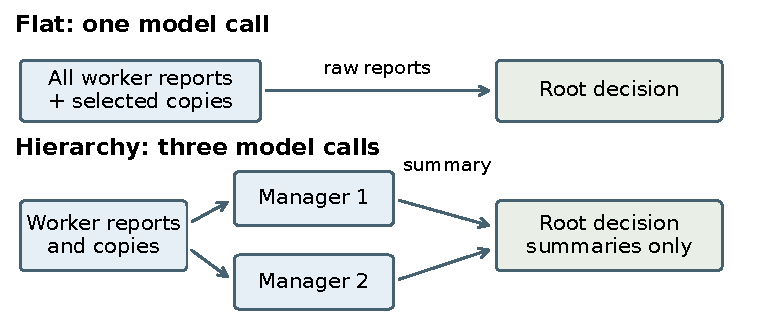
\includegraphics[width=\linewidth]{aggregation-architecture.pdf}
\caption{Flat and hierarchical replay. Copies repeat existing information without adding sources or running workers again.}
\label{fig:architecture}
\end{figure}

Figure \ref{fig:architecture} shows the difference in information access.
The flat decision maker reads all reports in one model call. In the hierarchy,
two managers summarize assigned groups of reports for a final decision maker,
requiring three calls in total. Copies stay with the manager receiving the
original report. The final decision maker receives the summaries and a list of
what the reports must cover and where they originated. This list supplies neither
the original findings nor the correct answer.

We compare three decision policies using the same evidence and selection rule.
Ordinary synthesis asks the model to combine the reports. A required-task
checklist explicitly asks it to check mandatory requirements before comparing
objectives. Scope-aware consolidation also asks it to combine equivalent claims,
keep differences in entity, condition, or version distinct, and flag unresolved
conflicts. It receives no additional correctness labels. Because this policy adds
instructions as well as guidance on handling sources, their effects cannot be
separated.

All policies follow the same output format. Managers report findings, what each
finding applies to, and unresolved items. Final decision makers return candidate
assessments, a choice, probabilities, and supporting claims. Even ordinary
synthesis therefore receives guidance to separate feasibility from the objective.
Output constraints enforce JSON structure but allow objective fields to contain
values other than numbers. The analysis evaluates reported values and decisions,
not private reasoning.



\subsection{Models, Evaluation Stages, and Scope}
The evaluation combines systematic testing across two models with focused
investigations of how information is preserved and used. Its contribution is
to connect overall decision performance with checks of what reaches the final
decision maker, allowing failures hidden by aggregate accuracy to be examined
directly.

We evaluate Qwen3-14B \cite{qwenmodel}, with thinking disabled, and Phi-4
\cite{phimodel}. Both run sequentially in bfloat16 without quantization on
RTX 6000 Ada Generation GPUs. Model weights, tokenizer revisions, native chat
templates, and decoding settings remain fixed. Sampling uses temperature 0.3,
top-$p$ 0.95, a 12,288-token context limit, a 2,304-token output cap, and batches
of up to 32. Appendix \ref{app:reproducibility} provides versions and details
of the checkpointed hardware continuation.

% BEGIN AUTO: stage-table
\begin{table}[htbp]
\centering\small
\setlength{\tabcolsep}{4pt}
\caption{Evaluation stages. Base problems are shared across models. Calls count accepted executions.}\label{tab:stages}
\begin{tabular}{llrrrr}\toprule
Stage & Models & Bases & Sched. & Trajectories & Calls\\\midrule
Pilot & Qwen3 & 24 & 12 & 1,152 & 2,304\\
Validation & Both & 36 & 18 & 5,184 & 10,368\\
Main held-out & Both & 192 & 96 & 27,648 & 55,296\\
Mechanism held-out & Qwen3 & 48 & 24 & 576 & 1,152\\
Root diagnostic & Qwen3 & 6 reused & 6 & 192 & 192\\
\bottomrule\end{tabular}
\end{table}
% END AUTO: stage-table

Table \ref{tab:stages} shows how the study progresses from development to
held-out evaluation and targeted diagnosis. The main experiment contains
$192\times2\times3\times2\times3\times2\times2=27{,}648$ decision trajectories,
covering paired worlds, report presentations, organizations, decision policies,
models, and stochastic generations. Using the same base problems across these
conditions supports direct comparisons, with 192 base pairs providing the
independent units of evaluation. Half the trajectories require one model call
and half require three, producing 55,296 accepted calls. The mechanism study
reuses some manager outputs across access conditions, so its call count reflects
actual executions rather than separate full runs of every trajectory.

The staged design also tests whether promising development findings extend
beyond the examples that motivated them. The pilot uses two policies, while
validation and main evaluation use three. Comparisons across stages retain
ordinary synthesis and checklist conditions to keep the policies matched.
The main headline results cover all three policies.

Both models passed the original 85\% development competence gate on flat,
unrepeated, ordinary-synthesis cases. Scheduling accuracy was 97.92\% for Qwen3
and 100\% for Phi-4. Workflow accuracy was 87.50\% and 93.75\%, respectively.
These checks established that the models and interfaces could perform the tasks
before the main evaluation. They did not guarantee held-out performance or
provide grounds for excluding later results. The frozen allocation retained
192 pairs using complete validation results and measured runtime projections,
without outcome-based stopping.

The initial research questions and analysis were fixed in the repository before
main inference. A dated amendment introduced the pilot-inspired mechanism study
while preserving the original design and without inspecting partial main
outcomes. Separate validation selected 48 fresh pairs under a prospective
precision and runtime rule. These records document when decisions were made,
although the study was not externally preregistered. Pilot-inspired trace
analyses and the transition analysis added during this revision remain
exploratory.

The completed evidence brings together the main replay evaluation, development
audits, a direct diagnostic of final-stage decisions, and a separate held-out
mechanism study. This combination supports an assessment of repetition that
examines both outcomes and the information available when decisions are made.
Supporting and live-worker comparisons were not completed for both models,
and the planned objective-only repair replay and balanced-objective confirmation
are outside this version's evidence. Specific effects of numerical repair,
provenance, report position, and worker scaling therefore remain unresolved.
No partial two-model supporting results enter the reported estimates.



\subsection{Outcomes, Pairing, and Uncertainty}
Exact agreement with the deterministic answer is primary. Malformed or truncated
responses count as operational errors, including manager failures followed by
correct final choices. Failures are not resampled, and all planned main calls
are complete.

For each model, we average accuracy within each base over worlds, policies,
organizations, and generations. Matched comparisons across $B$ independent
bases estimate the repetition effect
\begin{equation}
 \Delta_r=\frac{1}{B}\sum_{b=1}^{B}
 \left(\bar Y_{b,r}-\bar Y_{b,\mathrm{single}}\right).
\label{eq:effect}
\end{equation}
Positive values indicate improvement and reverse the original error-based harm
sign. We test whether hierarchy changes repetition's effect by subtracting the
flat effect from the hierarchical effect, averaging exact and paraphrased
repetition.

Paired-world success requires both answers to be correct, testing responsiveness
to consequential edits and stability under harmless edits. Predeclared contrasts
compare repetition effects between these outcomes. They also compare
scope-aware consolidation with the checklist on accuracy in repeated
consequential cases and changed-claim retention in hierarchical consequential
cases. Scheduling is primary. Workflow and other identified analyses are
secondary or exploratory.

Uncertainty estimates preserve dependence among related runs. We use 10,000
bootstrap draws of whole base problems, stratified by mutation family and
decision-change status \cite{clusterbootstrap}. Each draw retains all associated
conditions and generations. Models are reported separately with pointwise 95\%
intervals, without simultaneous coverage or multiplicity adjustment.
No confirmatory $p$-values are reported. The manifest requires Holm adjustment
across six primary contrasts if such tests are added. Intervals spanning zero
do not establish equivalence. The six-base root diagnostic reports counts
because its strata cannot support useful intervals.









\section{Main Held-Out Results}
\subsection{Accuracy and Organizational Structure}
Table \ref{tab:headline} quantifies the contribution of repetition while holding
problems and essential information fixed, using 2,304 trajectories per arm and
96 independent bases. Across both models, the results provide a practical
benchmark for repetition strategies, showing small average changes without a
reliable accuracy gain under this interface.

% BEGIN AUTO: main-headline
\begin{table}[htbp]
\centering\small
\setlength{\tabcolsep}{4pt}
\caption{Primary scheduling accuracy and paired changes. Each arm has 96 bases and 2,304 trajectories.}\label{tab:headline}
\begin{tabular}{llrrr}\toprule
Model & Repetition & Single \% & Repeated \% & Change, pp [95\% CI]\\\midrule
Qwen3-14B & exact & 88.72 & 88.54 & -0.17 [-2.21, +1.74]\\
Qwen3-14B & paraphrase & 88.72 & 88.24 & -0.48 [-2.39, +1.35]\\
Phi-4 & exact & 80.03 & 78.95 & -1.09 [-3.17, +1.00]\\
Phi-4 & paraphrase & 80.03 & 80.73 & +0.69 [-1.09, +2.52]\\
\bottomrule\end{tabular}
\end{table}
% END AUTO: main-headline

\begin{figure}[htbp]
\centering
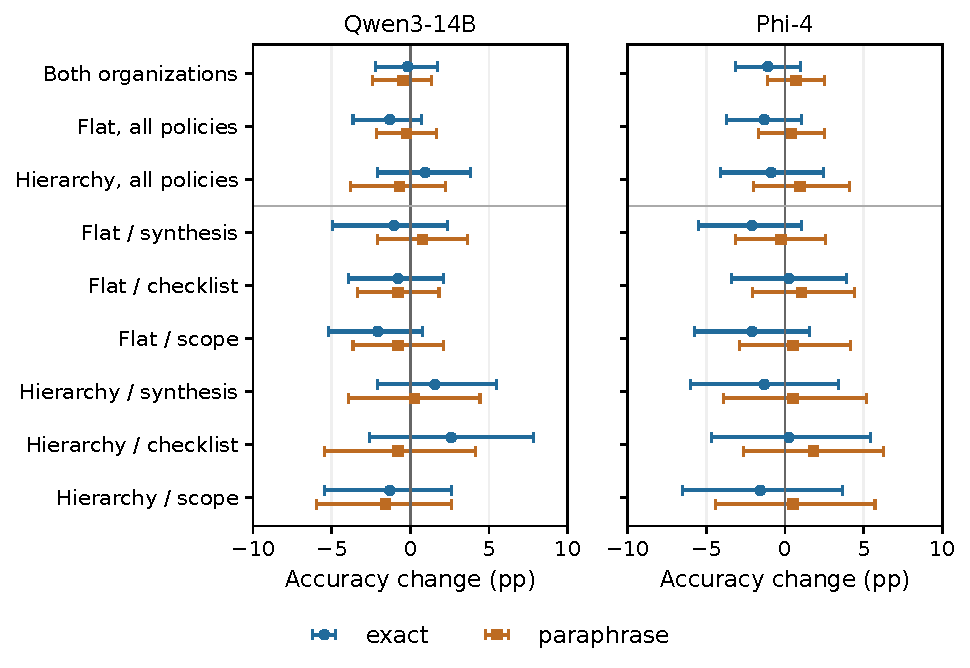
\includegraphics[width=\linewidth]{heldout-repetition-effects.pdf}
\caption{Scheduling accuracy changes, repeated minus single. Bars are pointwise 95\% intervals over 96 bases.}
\label{fig:effects}
\end{figure}

Figure \ref{fig:effects} places overall effects alongside organization and policy
breakdowns, revealing variation in the direction of the estimates. These
comparisons help identify settings for closer investigation, although their
shared bases mean they are not independent replications.

% BEGIN AUTO: organization-findings
For Qwen3-14B, unrepeated accuracy is 92.97\% in the flat organization and 84.46\% in the hierarchy. The hierarchical exact-copy effect is +0.95 [-2.08, +3.82] percentage points. The prespecified hierarchy interaction, averaging exact copies and paraphrases, is +0.91 [-2.17, +3.99] points on the accuracy scale.

For Phi-4, unrepeated accuracy is 88.80\% in the flat organization and 71.27\% in the hierarchy. The hierarchical exact-copy effect is -0.87 [-4.08, +2.43] percentage points. The prespecified hierarchy interaction, averaging exact copies and paraphrases, is +0.48 [-3.08, +4.17] points on the accuracy scale.
% END AUTO: organization-findings

The baseline accuracy gaps make hierarchical information delivery an important
target for diagnosis. The interaction intervals nevertheless do not establish
that hierarchy consistently changes repetition's effect. Because hierarchy
changes information access and call count together, the gaps cannot be
attributed to agent count alone.

% BEGIN AUTO: policy-findings
For Qwen3-14B, scope-aware consolidation minus the checklist changes accuracy on repeated consequential scheduling cases by -0.39 [-3.91, +3.26] points. Its change in retention of altered claims across all hierarchical consequential cases is -0.78 [-3.39, +1.22] points. Each comparison uses 48 independent bases.

For Phi-4, scope-aware consolidation minus the checklist changes accuracy on repeated consequential scheduling cases by -1.30 [-5.34, +2.86] points. Its change in retention of altered claims across all hierarchical consequential cases is -3.12 [-5.27, -1.13] points. Each comparison uses 48 independent bases.
% END AUTO: policy-findings

These comparisons demonstrate the value of measuring information preservation
alongside accuracy. Richer consolidation instructions provide no clear accuracy
advantage over the checklist, while Phi-4's lower retention estimate identifies
a specific weakness in preserving changed claims. More detailed instructions
therefore require direct evaluation of what survives summarization.
All policies already share the registry and structured output support.
Appendix \ref{app:policies} reports absolute accuracies for each condition.





\subsection{Consequential Changes and Harmless Controls}
Table \ref{tab:paired} requires correctness before and after the world edit.
A correct answer in just one world is a failure on this stricter outcome.
The exact-copy pattern differs across models and edit classes, and the
predeclared difference of effects uses both repetition forms.

% BEGIN AUTO: paired-results
\begin{table}[htbp]
\centering\small
\setlength{\tabcolsep}{4pt}
\caption{Both worlds correct (\%), scheduling. Each row has 48 bases and 576 paired cells per arm.}\label{tab:paired}
\begin{tabular}{llrrrr}\toprule
Model & Edit & Single & Exact & Para. & Exact change, pp [95\% CI]\\\midrule
Qwen3-14B & harmless & 80.03 & 78.12 & 78.12 & -1.91 [-6.08, +1.91]\\
Qwen3-14B & consequential & 83.85 & 88.37 & 86.63 & +4.51 [+0.52, +8.51]\\
Phi-4 & harmless & 68.75 & 71.01 & 71.01 & +2.26 [-1.56, +6.08]\\
Phi-4 & consequential & 72.57 & 70.14 & 73.26 & -2.43 [-6.25, +1.39]\\
\bottomrule\end{tabular}
\end{table}

For Qwen3-14B, the direct consequential-minus-harmless difference in the repetition effect on paired success is +5.56 [+0.09, +11.20] points, averaging exact and paraphrased repetition. For Phi-4, the direct consequential-minus-harmless difference in the repetition effect on paired success is -3.12 [-7.90, +1.74] points, averaging exact and paraphrased repetition.
Qwen3's contrast favors consequential pairs, whereas Phi-4's interval includes
either direction. This is neither a shared tendency to ignore changes nor evidence
of equivalent sensitivity. The test concerns response to a world edit. Identifying
loss of an exception within one input requires a separate claim-level test.


\subsection{Corrections, Regressions, and Stochastic Variation}
The transition analysis reveals changes in decision reliability that average
accuracy conceals. Table \ref{tab:transitions} separates corrected mistakes,
newly introduced mistakes, and changes between incorrect answers. Qwen3's
93 corrections and 97 regressions produce a net loss of only four correct
decisions out of 2,304. The small average effect therefore masks considerable
movement in which decisions succeed. Changes between incorrect answers reveal
further sensitivity that an accuracy comparison cannot capture.

% BEGIN AUTO: transition-results
\begin{table}[htbp]
\centering\small
\setlength{\tabcolsep}{4pt}
\caption{Scheduling transitions. Answer changes require two valid trajectories; counts are paired comparisons.}\label{tab:transitions}
\begin{tabular}{llrrrrr}\toprule
Model & Comparison & N & Corrected & Spoiled & Wrong/wrong & Answer changes\\\midrule
Qwen3-14B & Single, 0 to 1 & 1152 & 28 & 28 & 7 & 62/1151\\
Qwen3-14B & Exact, 0 to 1 & 1152 & 31 & 25 & 4 & 60/1152\\
Qwen3-14B & Single to exact & 2304 & 93 & 97 & 24 & 213/2303\\
Phi-4 & Single, 0 to 1 & 1152 & 70 & 66 & 15 & 148/1149\\
Phi-4 & Exact, 0 to 1 & 1152 & 97 & 60 & 22 & 177/1149\\
Phi-4 & Single to exact & 2304 & 143 & 168 & 51 & 357/2298\\
\bottomrule\end{tabular}
\end{table}

Qwen3-14B has 93 corrections and 97 regressions under exact repetition. Its within-condition answer-change rate is 5.38\% without repetition and 5.21\% with exact repetition. The latter minus the former is -0.17 [-1.74, +1.39] percentage points.

Phi-4 has 143 corrections and 168 regressions under exact repetition. Its within-condition answer-change rate is 12.85\% without repetition and 15.36\% with exact repetition. The latter minus the former is +2.52 [+0.61, +4.51] percentage points.
% END AUTO: transition-results

\begin{figure}[htbp]
\centering
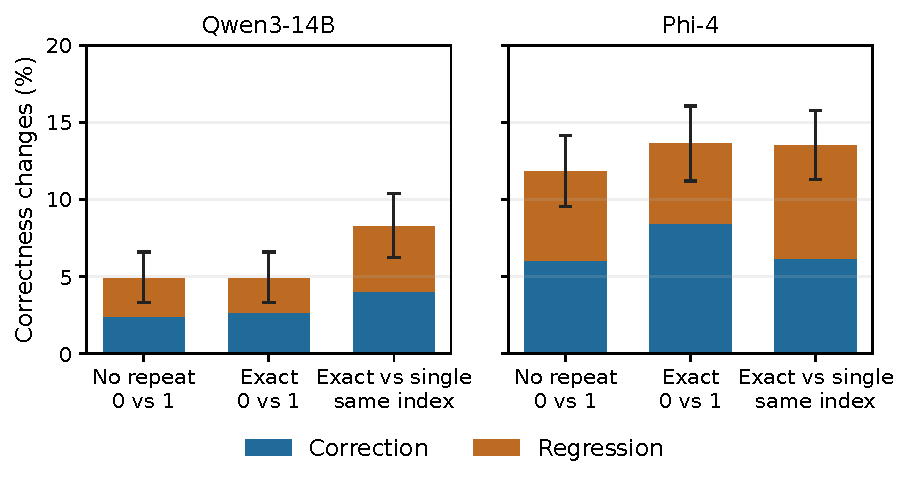
\includegraphics[width=\linewidth]{correctness-transitions.pdf}
\caption{Corrections and regressions in scheduling. Bars show 95\% base-cluster intervals for total correctness changes.}
\label{fig:transitions}
\end{figure}

Figure \ref{fig:transitions} distinguishes variation between repeated runs from
changes between presentation conditions. The first two comparisons match
generations 0 and 1 within a condition, giving 1,152 pairs per model. The third
compares single and exact presentations at matching generation indices, giving
2,304 pairs. Seeds are shared across conditions for each base, generation index,
and stage. Within-condition comparisons therefore use different seeds, whereas
cross-condition comparisons use common seeds. This distinction matters because
the larger cross-condition count alone cannot establish increased stochastic
instability.

Comparing within-condition disagreement provides a more direct assessment of
repeatability. Qwen3's estimate is near zero and uncertain, while Phi-4 shows
greater disagreement under exact repetition in this exploratory analysis.
This result demonstrates the value of measuring consistency alongside accuracy.
There is only one different-seed pair per world, policy, and organization.
Rates use all paired cells and count answer changes only when both trajectories
are valid, with valid-answer denominators listed separately. The combined
analysis makes both corrected decisions and reduced repeatability visible,
providing a more informative assessment of repetition within the tested settings.




\subsection{Generalization Beyond the Pilot}
% BEGIN AUTO: stage-comparison
Under the shared synthesis/checklist policies, the hierarchical Qwen3 exact-copy effect is +13.54 [+4.17, +22.92] points in the 12-base pilot, -3.47 [-10.42, +2.78] in the 18-base validation subset, and +2.08 [-1.56, +5.60] in the 96-base main subset. These averages retain both worlds and both stochastic generations. The main two-policy estimate therefore differs from the three-policy headline. One pilot base contributes seven of 14 corrections. It remains included in every primary estimate. The pilot pattern is less pronounced in the later evaluations, which also change graph patterns, parameter combinations, and language templates. This establishes a limit on generalization of the development finding, without identifying which changed feature explains it.
% END AUTO: stage-comparison

Figure \ref{fig:cases} in the appendix displays every main scheduling base in a
fixed identifier order. Positive and negative effects occur across problems,
without selecting exclusions or a favorable subpopulation. The main inference
continues to weight each independent base equally.




\subsection{Secondary Workflow Findings}
The workflow evaluation extends the study to conditions, quantifiers, and version
rules, testing repetition beyond numerical scheduling constraints.
Table \ref{tab:workflow} identifies a practically important risk for Phi-4,
with accuracy decreasing under both exact copies and paraphrases. Qwen3's
estimates remain close to zero with uncertain direction. These results broaden
the assessment of repetition while preserving workflow as a distinct secondary
population with the same feasibility-before-objective decision structure.

% BEGIN AUTO: workflow-results
\begin{table}[htbp]
\centering\small
\setlength{\tabcolsep}{4pt}
\caption{Secondary workflow accuracy. Each arm has 96 bases and 2,304 trajectories.}\label{tab:workflow}
\begin{tabular}{llrrr}\toprule
Model & Repetition & Single \% & Repeated \% & Change, pp [95\% CI]\\\midrule
Qwen3-14B & exact & 78.69 & 78.91 & +0.22 [-2.17, +2.43]\\
Qwen3-14B & paraphrase & 78.69 & 78.52 & -0.17 [-2.26, +1.82]\\
Phi-4 & exact & 74.65 & 71.66 & -2.99 [-5.03, -1.09]\\
Phi-4 & paraphrase & 74.65 & 71.79 & -2.86 [-5.03, -0.78]\\
\bottomrule\end{tabular}
\end{table}
% END AUTO: workflow-results

Both models passed the original development gate. On held-out flat, unrepeated,
ordinary-synthesis workflow cases, accuracy reaches 84.38\% for Qwen3 and
83.33\% for Phi-4, below the 85\% reference. Retaining these cases documents
the challenge of generalizing beyond development examples, without removing
a difficult task or retuning models after testing. The lower competence limits
interpretation, but the results identify a concrete setting where repeated
presentation can undermine decision quality. The intervals remain pointwise
and secondary, providing evidence for targeted investigation rather than a
family-wide confirmatory significance claim.





\section{Information Preservation and Decision Sufficiency}
\label{sec:preservation}

\subsection{Where Numerical Information Changes}
The pipeline audit traces typed reports, manager inputs, raw and parsed summaries, and actual root inputs across 60 independent pilot and validation bases, 3,168 hierarchical trajectories, and 6,336 manager summaries. Checked values remain unchanged through parsing and delivery. Numerical objectives replaced by Boolean \texttt{true} already appear in generated summaries, locating the loss at communication rather than subsequent processing.

This distinguishes format compliance from meaning preservation. Although prompts request numerical objectives, the shared assertion schema permits Boolean and numerical values without tying types to reported properties. A compliant summary can therefore discard a necessary comparison. Replacing makespans of 3 and 5 with \texttt{true}, for example, erases their ordering. Whether this changes the answer depends on remaining evidence, including feasibility, motivating separate measures of information preservation and decision sufficiency.

% BEGIN AUTO: numeric-results
\begin{table}[htbp]
\centering\small
\setlength{\tabcolsep}{4pt}
\caption{Objective-field audit. Entries give single / exact counts; field denominators are per arm.}\label{tab:numeric}
\begin{tabular}{lrrrr}\toprule
Scheduling subset & Fields & Preserved & Boolean & Omitted\\\midrule
Pilot Qwen3 & 288 & 219 / 270 & 60 / 9 & 9 / 9\\
Validation Qwen3 & 648 & 561 / 549 & 53 / 64 & 34 / 35\\
Validation Phi-4 & 648 & 458 / 449 & 156 / 156 & 25 / 40\\
\bottomrule\end{tabular}
\end{table}
% END AUTO: numeric-results

\begin{figure}[htbp]
\centering
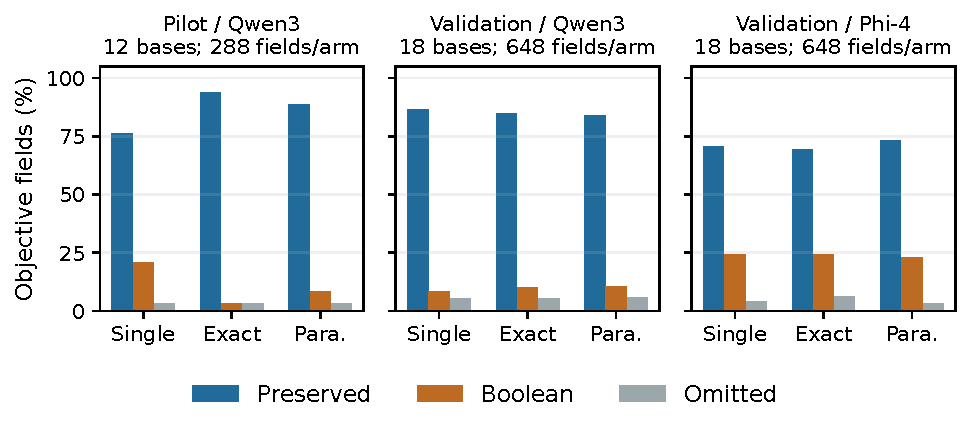
\includegraphics[width=\linewidth]{numerical-fidelity.pdf}
\caption{Objective fidelity in the development audit. Counts use distinct scoped fields, not repeated copies.}
\label{fig:fidelity}
\end{figure}

Table \ref{tab:numeric} and Figure \ref{fig:fidelity} quantify this loss. Exact repetition reduces Boolean replacements from 60 to 9 in the Qwen3 pilot, but validation does not consistently reproduce this pattern. Repetition therefore cannot be assumed to preserve numerical meaning. The pilot averages two policies and validation three, preventing isolation of an evaluation-stage effect. Preservation requires the correct value, candidate, and property without unresolved conflict. Displayed categories are neither exhaustive nor mutually exclusive; correct but unresolved values do not count as preserved.

In the pilot base contributing most to corrections, all eight baseline objective-bearing summaries replace numbers with Booleans, while all eight exact-copy summaries preserve them. The repeated report concerns a nonwinning candidate. Selected for its contribution, this case illustrates a possible process rather than its frequency; aggregate rates and intact controls supply context. The reproducibility record also retains a fixed, identifier-ordered selection of Boolean-loss, omission, altered-value, and intact traces where available.

Requiring numerical objective fields could reject Boolean substitutions without guaranteeing correct values or candidate associations. Whether alternative schemas, examples, or models improve decisions remains untested. The audit establishes how to locate semantic information loss and distinguish it from transport errors and failures to use preserved information.






\subsection{Separating Information Loss from Decision Failure}
We test whether the information an agent receives sufficiently supports its decision. Missing information need not create uncertainty: if only one candidate is feasible, its missing completion time may not affect the choice. Conversely, sufficient information does not guarantee a correct decision. We distinguish representation fidelity (preserving values and scope), decision sufficiency (whether visible information determines one answer), and final accuracy (agreement with the actual world).

The support scorer fixes supplied, uncontested values and considers all admissible completions of unknown fields. Mandatory requirements are Boolean; objectives are nonnegative integers. It enumerates feasibility combinations and objective orderings, including ties. Information uniquely supports a choice only if every completion yields that answer. The scorer uses the public report interface without importing evaluator truth or hidden schedule details.

Contradictory or incorrectly typed fields remain flagged as representation errors. A complementary analysis treats these fields as unknown and tests whether every admissible replacement leaves the answer unchanged. This distinguishes representation damage from decision ambiguity without repairing or validating erroneous contents.

% BEGIN AUTO: sufficiency-results
\begin{table}[htbp]
\centering\small
\setlength{\tabcolsep}{4pt}
\caption{Decision support from uncontested summary fields. Representation-error cases remain flagged.}\label{tab:sufficiency}
\begin{tabular}{lrrrr}\toprule
Scheduling subset & Trajectories & Unique choice & With invalid fields & Violations\\\midrule
Pilot Qwen3 & 288 & 248 & 8 & 4\\
Validation Qwen3 & 648 & 585 & 40 & 73\\
Validation Phi-4 & 648 & 411 & 39 & 52\\
\bottomrule\end{tabular}
\end{table}
% END AUTO: sufficiency-results

Table \ref{tab:sufficiency} aggregates all three presentation conditions. Validation evidence uniquely supports a choice in 585 Qwen3 and 411 Phi-4 trajectories, yet valid final choices violate that support in 73 and 52 cases, respectively. These failures to follow available evidence escape summary-completeness checks and measure supported-choice agreement separately from world accuracy. Invalid-field counts are subsets of uniquely supported cases. The pilot uses two policies; validation uses three. Because repetition can affect information preservation, these conditional counts describe observed behavior rather than estimate causal mediation.



\subsection{Fixed-Summary Root Replay and Lossless Delivery}
The diagnostic uses six reused development pairs, both worlds, eight treatments,
and two delivery modes, producing 192 fresh root calls. Each combination receives
one call with fixed synthesis and output requirements. Treatments repeat one
objective, all objectives, or an existing constraint, alongside neutral and
position controls. There is no paraphrase arm.

Within each delivery mode, repetition preserves the distinct claims. Lossless
delivery carries the original worker assertions available to each branch,
preserving values and scopes without adding observations or hidden answers.
It can restore missing information and changes its presentation, so it does not
isolate numerical repair. Historical or deterministic manager processing is
excluded from the 192 fresh calls.

% BEGIN AUTO: root-results
Without repetition, frozen summaries yield 8/12 correct decisions and lossless
delivery yields 12/12. Ten frozen contexts uniquely support a choice, including
two with irrelevant invalid objective fields. The root violates that supported
choice twice. The other two contexts remain underdetermined. Both delivery modes
average 3,333 input tokens.

Repeating all objectives already present in frozen summaries also yields 12/12
correct decisions, but only ten are uniquely supported. Existing Boolean values
are repeated without restoring missing numbers. Lossless delivery achieves 12/12
with and without repetition. Individual-objective and neutral-material treatments
include regressions, detailed in Appendix \ref{app:root}.
% END AUTO: root-results

\begin{figure}[htbp]
\centering
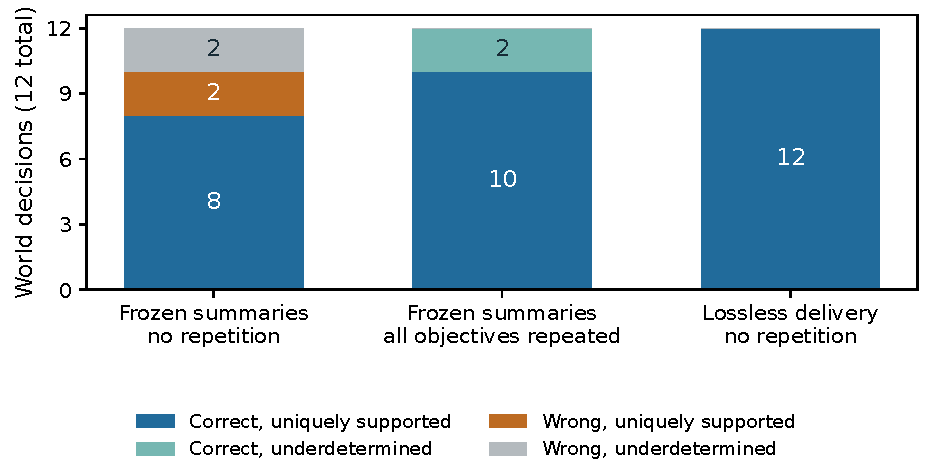
\includegraphics[width=\linewidth]{root-delivery-diagnostic.pdf}
\caption{Root diagnostic on 12 worlds from six bases. World correctness and uniquely supported correctness differ.}
\label{fig:root}
\end{figure}

Figure \ref{fig:root} highlights two routes to 12/12 accuracy with different
evidential support. Only lossless delivery makes every choice uniquely justified
by the visible information. These six reused bases illustrate observable failure
locations without establishing precise population effects, complete causal
mediation, or the model's hidden reasoning.





\subsection{A Separate Test of Repetition Targets and Raw-Report Access}
Using 48 fresh pairs and 576 trajectories, this Qwen3 study tests two practical
design choices, which reports to repeat and whether to expose original reports.
Half the pairs concern each task. Executable rules identify correct mandatory
findings whose isolated truth-value flip changes the answer as decisive.
Common targets are true favorable findings for infeasible candidates when
available, otherwise correct nondecisive Boolean findings. Targets are selected
before inference and may differ between worlds.

Six arms compare no repetition, common, decisive, or uniform repetition, and
raw-report access with or without common repetition. Raw-access arms reuse the
corresponding manager summaries and expose evidence already available to managers.

% BEGIN AUTO: mechanism-results
\begin{table}[htbp]
\centering\small
\setlength{\tabcolsep}{4pt}
\caption{Separate Qwen3 mechanism test. Each task has 24 fresh bases and 48 decisions per arm.}\label{tab:mechanism}
\begin{tabular}{lrrr}\toprule
Arm & Schedule \% & Workflow \% & Sched. retention \%\\\midrule
No repetition & 87.50 & 83.33 & 95.83\\
Common finding, four & 87.50 & 75.00 & 95.57\\
Decisive finding, four & 85.42 & 91.67 & 99.11\\
All reports, four each & 79.17 & 70.83 & 96.09\\
Raw access, no repetition & 85.42 & 83.33 & 95.83\\
Raw access, common four & 81.25 & 72.92 & 95.57\\
\bottomrule\end{tabular}
\end{table}

The prespecified scheduling contrasts are -2.08 [-10.42, +6.25] points for
decisive versus common repetition, -0.26 [-0.78, 0.00] for retention of unrepeated
necessary claims under common repetition, and +4.17 [-4.17, +10.42] for the
repetition-by-access interaction. These provide direct tests of strategies for
preserving decision-relevant information. Accuracy contrasts remain uncertain,
and the small retention estimate does not establish equivalence.

Uniform repetition produces a substantial observed workflow decline, from
83.33\% to 70.83\%, or -12.50 [-20.83, -4.17] points. This identifies a concrete
setting where repeating all reports reduces decision quality. The comparison
is secondary and uses one model. Repetition also lengthens the input, so the
result does not isolate context length or establish general harm to exception
handling.
% END AUTO: mechanism-results

Table \ref{tab:mechanism} makes information preservation visible alongside
accuracy. Retention averages each trajectory's fraction of eligible, unrepeated
necessary claims preserved with correct values and scopes, without contradictions
or unresolved flags. Removing a necessary claim makes the decision undetermined.
Missing values count as losses. Other arm comparisons and all workflow effects
are secondary.




\section{Discussion and Limitations}
The study evaluates agent communication through information preservation, decision
sufficiency, and correct application. Across two models and 192 independent base
pairs, small average scheduling effects conceal corrections and regressions,
while secondary workflow results identify accuracy losses. Comparing these
transitions with ordinary sampling variation avoids treating every answer
change as instability.

Audits locate numerical objective loss in raw manager responses, with no
subsequent changes during parsing or delivery. Scope-dependent type checks could
reject Boolean objectives, although their decision benefit remains untested.
The six-pair diagnostic shows why accuracy alone is insufficient. Missing facts
can leave a choice determined, and correct answers can lack adequate support.
These distinctions could guide source retrieval and decision validation.

The synthetic tasks and frozen correct reports isolate aggregation, with
deployment failures, autonomous worker errors, and error independence outside
the established evidence. Workflow shares scheduling's selection structure.
Organization changes access and call count together, while raw access and
uniform repetition also alter input length. Incomplete controls for call count,
length, ancestry, and live workers limit attribution.

Both models use fixed precision, decoding, and structured outputs. Shared
candidate-assessment guidance narrows policy differences, and scope-aware
consolidation also adds instructions. Generalization to other models, reasoning
modes, free-form communication, deeper organizations, and feedback remains open.

The main contrasts were frozen before inference, while pilot-inspired audits
and transition analyses remain exploratory. Pointwise intervals do not establish
family-wise significance. The six-pair diagnostic and 24 scheduling pairs in
the extension limit precision, and no equivalence margin was prespecified.
Traces locate observable failures without establishing causal mediation or
private reasoning. Within these boundaries, the framework provides concrete
criteria for testing whether communication improvements preserve evidence
and support justified decisions.


\section{Conclusion}
This study provides a controlled framework for following information from repeated reports to final decisions. Across two models and 192 independent held-out base pairs, small, uncertain scheduling effects do not reproduce the large pilot gain. Corrections and regressions reveal changes hidden by average accuracy, while secondary workflow and targeted findings identify settings where repetition reduces accuracy. Audits locate numerical-to-Boolean changes in raw summaries, and the exploratory root diagnostic separates information loss from failures to use sufficient evidence. Together, these contributions make representation fidelity, decision sufficiency, and final accuracy separately measurable. They give future agent frameworks a practical basis for testing whether communication changes preserve required values and scopes and whether those improvements translate into better decisions.


\FloatBarrier
\clearpage
\appendix
\section{Reproducibility and Output Semantics}
\label{app:reproducibility}
The accompanying materials contain generators, independent verifiers, templates,
frozen configurations, immutable requests and responses, and analysis scripts.
All reported tables and figures are generated from complete local records.
Identifying repository links are omitted for anonymous review. Original analyses
are preserved alongside an analysis-only correction that sorts cluster identifiers
before bootstrap resampling. That correction changes Monte Carlo endpoints for
the hierarchy interaction, not the decisions, estimator, strata, or experiment.
The bootstrap seed is 20271015. The frozen model-averaging rule gives each model
equal weight, while this paper presents model-specific estimates.

Model and tokenizer revisions are identical within each family. Qwen3-14B uses
\begin{quote}\small\texttt{40c069824f4251a91eefaf281ebe4c544efd3e18}\end{quote}
and Phi-4 uses
\begin{quote}\small\texttt{2db69c1c3e91a05d2c64a3185acfbaf36f744e25}\end{quote}
Their licenses are Apache 2.0 and MIT. The environment uses vLLM 0.10.2,
PyTorch 2.8.0 with CUDA 12.8, and Transformers 4.55.4. Checkpointed continuation
used RTX 6000 Ada Generation hardware with 49,140 MiB memory. Recorded driver
versions are 595.91.07 and 570.124.06 across the original and replacement
allocations. Frozen model, prompt, precision, and sampling settings were retained.
Prefix caching is disabled. Native chat-template token IDs are submitted directly,
with template dates pinned to 16 October 2026. Seeds derive from base identifier,
generation index, and stage. Distinct generation indices retain distinct requests.

Manager assertions are triples of scope key, value, and cited report identifiers,
for example \texttt{["objective|P|...", 3, ["report-id"]]}. The surrounding
JSON also lists unresolved keys. Roots add candidate assessments, a choice, and
probabilities. The scope registry carries units and applicability. A Boolean is
never scored as a valid numerical objective. Integral floats such as 3.0 are
numerically equivalent to 3. Correctness includes operational failures as errors.
Invalid selections use all trajectories as the denominator, while calibration
requires a valid probability distribution and reports its available denominator
in the analysis files.

\section{Policy Breakdown and Resource Use}
\label{app:policies}
Table \ref{tab:policies} provides absolute scheduling accuracy for each policy.
These values explain why the pooled comparison should not be attributed to
provenance instructions alone. Scope-aware consolidation has no consistent
accuracy advantage across model and organization cells.

% BEGIN AUTO: policy-table
\begin{table}[htbp]
\centering\small
\setlength{\tabcolsep}{4pt}
\caption{Main scheduling accuracy (\%) by policy. Each cell has 96 bases and 384 trajectories.}\label{tab:policies}
\begin{tabular}{lllrrr}\toprule
Model & Organization & Policy & Single & Exact & Para.\\\midrule
Qwen3-14B & flat & synthesis & 91.15 & 90.10 & 91.93\\
Qwen3-14B & flat & checklist & 95.05 & 94.27 & 94.27\\
Qwen3-14B & flat & scope & 92.71 & 90.62 & 91.93\\
Qwen3-14B & hierarchy & synthesis & 87.76 & 89.32 & 88.02\\
Qwen3-14B & hierarchy & checklist & 78.65 & 81.25 & 77.86\\
Qwen3-14B & hierarchy & scope & 86.98 & 85.68 & 85.42\\
Phi-4 & flat & synthesis & 94.01 & 91.93 & 93.75\\
Phi-4 & flat & checklist & 89.06 & 89.32 & 90.10\\
Phi-4 & flat & scope & 83.33 & 81.25 & 83.85\\
Phi-4 & hierarchy & synthesis & 80.21 & 78.91 & 80.73\\
Phi-4 & hierarchy & checklist & 63.28 & 63.54 & 65.10\\
Phi-4 & hierarchy & scope & 70.31 & 68.75 & 70.83\\
\bottomrule\end{tabular}
\end{table}
% END AUTO: policy-table

Table \ref{tab:cost} counts input and output tokens, including the managers in a
hierarchical trajectory. Exact repetition adds processing even when average
accuracy does not improve. Allocated time is measured inference batch wall time
shared among requests, summed over the trajectory and divided by correct
answers. It excludes loading and setup, and is neither individual request
latency nor measured monetary cost. Shared manager calls in mechanism studies
are counted once in their physical inventories.

% BEGIN AUTO: cost-table
\begin{table}[htbp]
\centering\small
\setlength{\tabcolsep}{4pt}
\caption{Scheduling resources, single / exact. Time is allocated batch seconds per correct decision.}\label{tab:cost}
\begin{tabular}{llrrrr}\toprule
Model & Organization & Single tokens & Exact tokens & Single time & Exact time\\\midrule
Qwen3-14B & flat & 4,230 & 4,526 & 2.45 & 2.51\\
Qwen3-14B & hierarchy & 9,071 & 9,602 & 10.46 & 10.58\\
Phi-4 & flat & 3,709 & 3,967 & 2.14 & 2.26\\
Phi-4 & hierarchy & 8,001 & 8,455 & 10.21 & 10.61\\
\bottomrule\end{tabular}
\end{table}
% END AUTO: cost-table

\begin{figure}[htbp]
\centering
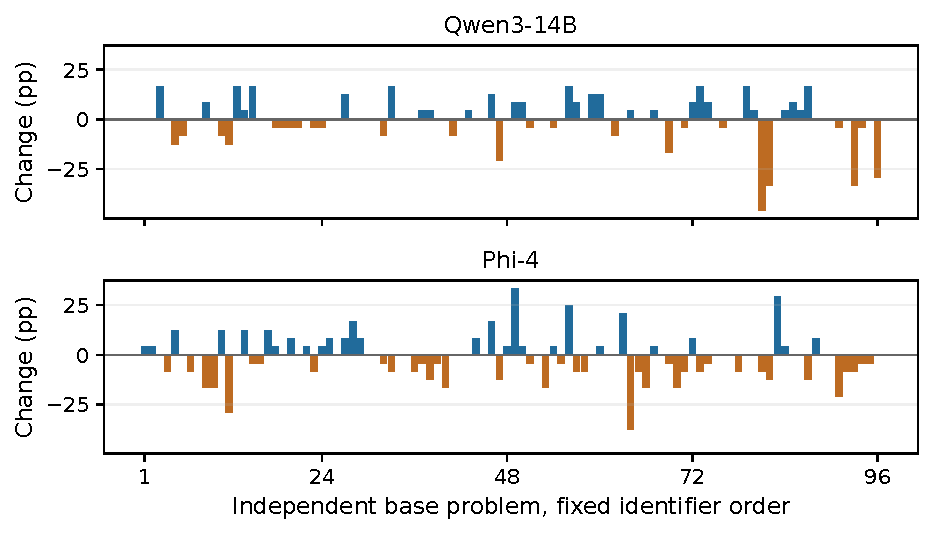
\includegraphics[width=\linewidth]{heldout-case-effects.pdf}
\caption{Exact-copy scheduling effects for all 96 bases. Each bar averages organizations, policies, worlds, and generations.}
\label{fig:cases}
\end{figure}

Figure \ref{fig:cases} shows how a small mean can conceal changes on individual
problems. Fixed identifier ordering includes every base. These descriptive
effects do not define new confirmation subsets.

\section{Complete Root-Diagnostic Arms and Fresh Verification}
\label{app:root}
Table \ref{tab:root-all} reports every root-diagnostic arm, with twelve world
decisions from the same six bases. Objectives 1 to 3 follow the prespecified
candidate ordering. Agreement is counted only where uncontested facts determine
a unique answer. That denominator remains ten under frozen summaries and twelve
under lossless delivery. Neutral material changes no task evidence. The end arm
moves copies of the designated objective assertion to the end.

% BEGIN AUTO: root-table
\begin{table}[htbp]
\centering\small
\setlength{\tabcolsep}{4pt}
\caption{All root-diagnostic arms. Agreement uses only uniquely determined contexts.}\label{tab:root-all}
\begin{tabular}{lrrrr}\toprule
Arm & Frozen correct & Agreement & Lossless correct & Agreement\\\midrule
No repetition & 8/12 & 8/10 & 12/12 & 12/12\\
Objective 1 & 9/12 & 9/10 & 11/12 & 11/12\\
Objective 2 & 9/12 & 9/10 & 12/12 & 12/12\\
Objective 3 & 9/12 & 9/10 & 12/12 & 12/12\\
Constraint & 9/12 & 9/10 & 12/12 & 12/12\\
All objectives & 12/12 & 10/10 & 12/12 & 12/12\\
Neutral material & 9/12 & 9/10 & 11/12 & 11/12\\
Objective at end & 8/12 & 8/10 & 11/12 & 11/12\\
\bottomrule\end{tabular}
\end{table}
% END AUTO: root-table

The lossless baseline's observed ceiling does not imply that its surrounding
prompt is immune to presentation changes. Individual-objective, position, and
neutral arms each include a wrong decision in at least one lossless context.
Uniform repetition under frozen summaries reaches twelve correct world answers
while two contexts remain underdetermined. The complete table prevents selecting
only the largest gain as evidence for a general repetition effect.

A separate six-base development verification probe completed 30 trajectories and
72 physical calls. Original reports, exact copies, paraphrases, added fresh
verification, and a fixed-allowance fresh variant all yielded six correct final
decisions out of six. Fresh checks corrected one initial worker error and also
introduced an incorrect finding. Roots had authoritative task data in every arm,
so their ceiling performance cannot be attributed solely to worker reports.
These calls share evidence sources and do not measure independent observations
or verified computational diversity. Their small sample supports a diagnostic
comparison rather than a worker-scaling conclusion.

\FloatBarrier
\begin{samepage}
  
\section*{Declaration on AI Assistance}
The author supplied the research direction and experimental requirements for the code development.
The AI coding assistant provided assistance with protocol implementation and methodological
refinements, software development and testing, experiment operation, literature
verification, statistical analysis, figure generation, and manuscript drafting.
No AI system is listed as an author. The author has reviewed and verified the manuscript, analyses, and reported results and takes responsibility for their accuracy and integrity.
\end{samepage}



\begin{thebibliography}{20}
\bibitem{sybil}
Bara, M.: Epistemic Sybil Resistance: Multiplying AI Agents Without Multiplying
Evidence. arXiv:2609.01873v1 (2026). Preprint.
\url{https://arxiv.org/abs/2609.01873v1}

\bibitem{mast}
Cemri, M., Pan, M.Z., Yang, S., Agrawal, L.A., Chopra, B., Tiwari, R., et al.: Why Do Multi-Agent LLM Systems Fail? Advances in Neural Information
Processing Systems \textbf{38}, Datasets and Benchmarks Track (2025).
\url{https://papers.nips.cc/paper_files/paper/2025/hash/b1041e52d3be19f0a9bc491657488e4a-Abstract-Datasets_and_Benchmarks_Track.html}

\bibitem{metadata}
Chiang, C.H., Lee, H.: Do Metadata and Appearance of the Retrieved Webpages Affect
LLM's Reasoning in Retrieval-Augmented Generation? In: Proceedings of the 7th
BlackboxNLP Workshop: Analyzing and Interpreting Neural Networks for NLP,
pp. 389--406 (2024). \url{https://doi.org/10.18653/v1/2024.blackboxnlp-1.24}

\bibitem{debate}
Du, Y., Li, S., Torralba, A., Tenenbaum, J.B., Mordatch, I.: Improving Factuality
and Reasoning in Language Models through Multiagent Debate. In: Proceedings of
the 41st International Conference on Machine Learning, PMLR 235,
pp. 11733--11763 (2024). \url{https://proceedings.mlr.press/v235/du24e.html}

\bibitem{clusterbootstrap}
Field, C.A., Welsh, A.H.: Bootstrapping clustered data. Journal of the Royal
Statistical Society: Series B (Statistical Methodology) \textbf{69}(3),
369--390 (2007). \url{https://doi.org/10.1111/j.1467-9868.2007.00593.x}

\bibitem{copies}
Gao, J., Li, R., Yu, T., Ren, L., Chen, B., Wang, Z.:
Copies or Sources? Measuring How LLM Aggregators Count Restated Evidence in
Multi-Agent Systems. arXiv:2610.06192v1 (2026). Preprint.
\url{https://arxiv.org/abs/2610.06192v1}

\bibitem{selfcorrect}
Huang, J., Chen, X., Mishra, S., Zheng, H.S., Yu, A.W., Song, X., et al.:
Large Language Models Cannot Self-Correct Reasoning Yet. In: International
Conference on Learning Representations (2024).
\url{https://proceedings.iclr.cc/paper_files/paper/2024/hash/8b4add8b0aa8749d80a34ca5d941c355-Abstract-Conference.html}

\bibitem{scaling}
Kim, Y., Gu, K., Park, C., Park, C., Schmidgall, S., Heydari, A.A., et al.:
Towards a Science of Scaling Agent Systems. arXiv:2512.08296v3 (2026).
Preprint, revised 8 April 2026. \url{https://arxiv.org/abs/2512.08296v3}

\bibitem{promptrepeat}
Leviathan, Y., Kalman, M., Matias, Y.: Prompt Repetition Improves Non-Reasoning
LLMs. arXiv:2512.14982v1 (2025). Preprint.
\url{https://arxiv.org/abs/2512.14982v1}

\bibitem{hidden}
Li, Y., Naito, A., Shirado, H.: Systematic Failures in Collective Reasoning under
Distributed Information in Multi-Agent LLMs. In: Proceedings of the 43rd
International Conference on Machine Learning, PMLR 306, pp. 69250--69268 (2026).
\url{https://proceedings.mlr.press/v306/li26ej.html}

\bibitem{middle}
Liu, N.F., Lin, K., Hewitt, J., Paranjape, A., Bevilacqua, M., Petroni, F., et al.: Lost in the Middle: How Language Models Use Long Contexts.
Transactions of the Association for Computational Linguistics \textbf{12},
157--173 (2024). \url{https://doi.org/10.1162/tacl_a_00638}

\bibitem{maynez}
Maynez, J., Narayan, S., Bohnet, B., McDonald, R.: On Faithfulness and Factuality
in Abstractive Summarization. In: Proceedings of the 58th Annual Meeting of the
Association for Computational Linguistics, pp. 1906--1919 (2020).
\url{https://doi.org/10.18653/v1/2020.acl-main.173}

\bibitem{phimodel}
Microsoft: Phi-4. Official model card, pinned revision listed in
Appendix \ref{app:reproducibility}. Accessed 18 October 2026.
\url{https://huggingface.co/microsoft/phi-4}

\bibitem{frank}
Pagnoni, A., Balachandran, V., Tsvetkov, Y.: Understanding Factuality in Abstractive
Summarization with FRANK: A Benchmark for Factuality Metrics. In: Proceedings of
the 2021 Conference of the North American Chapter of the Association for
Computational Linguistics: Human Language Technologies, pp. 4812--4829 (2021).
\url{https://doi.org/10.18653/v1/2021.naacl-main.383}

\bibitem{qwenmodel}
Qwen Team: Qwen3-14B. Official model card, pinned revision listed in
Appendix \ref{app:reproducibility}. Accessed 18 October 2026.
\url{https://huggingface.co/Qwen/Qwen3-14B}

\bibitem{checklist}
Ribeiro, M.T., Wu, T., Guestrin, C., Singh, S.: Beyond Accuracy: Behavioral
Testing of NLP Models with CheckList. In: Proceedings of the 58th Annual Meeting
of the Association for Computational Linguistics, pp. 4902--4912 (2020).
\url{https://doi.org/10.18653/v1/2020.acl-main.442}

\bibitem{smit}
Smit, A.P., Grinsztajn, N., Duckworth, P., Barrett, T.D., Pretorius, A.:
Should we be going MAD? A Look at Multi-Agent Debate Strategies for LLMs.
In: Proceedings of the 41st International Conference on Machine Learning,
PMLR 235, pp. 45883--45905 (2024).
\url{https://proceedings.mlr.press/v235/smit24a.html}

\bibitem{selfconsistency}
Wang, X., Wei, J., Schuurmans, D., Le, Q., Chi, E.H., Narang, S., et al.: Self-Consistency Improves Chain of Thought Reasoning in Language Models.
In: International Conference on Learning Representations (2023).
Camera-ready version: \url{https://arxiv.org/abs/2203.11171v4}

\bibitem{distributed}
Yan, C., Yue, Z., Zhao, F., Lin, E., Jia, L., Tong, H., et al.:
When Truth Is Distributed: Misinformation Derails Collective Fact Recovery in
LLM-Based Multi-Agent Systems. arXiv:2608.03421v1 (2026). Preprint.
\url{https://arxiv.org/abs/2608.03421v1}

\bibitem{paws}
Zhang, Y., Baldridge, J., He, L.: PAWS: Paraphrase Adversaries from Word Scrambling.
In: Proceedings of NAACL-HLT, Volume 1, pp. 1298--1308 (2019).
\url{https://doi.org/10.18653/v1/N19-1131}
\end{thebibliography}
\end{document}
